Consider a single cluster of radius $a$ irradiated with a short femtosecond pulse with $I_{h} \approx 10^{14}$ $\textrm{W/cm}^2$ intensity. The Drude model gives a representation of the plasma dielectric function:

    \begin{equation}
		\varepsilon (\omega) = 1 - {\left( \frac{\omega_{pe}}{\omega} \right)}^2 \frac{1}{1+i \beta_{e}}, \qquad \omega_{pe} = \sqrt{\frac{4 \pi e^2 n_e}{m_e}},
		\label{eps_plasma}
    \end{equation}
    \begin{equation*} % artificial indent after the equation
    \end{equation*}

\noindent where $\omega$ is the considered harmonic frequency, $\omega_{pe}$ is the electron plasma frequency, $n_e = Z n_i$ --- electron density, $Z$ is the average degree of ionization, $n_i$ is the ion density. $\beta_{e} = v_e / \omega$ and $v_e$ is the electron-ion collision coefficient in the Spitzer approximation. 

%Under solid-state plasma conditions, the cluster ion density is of the order of $n_i = 6 \cdot 10^{22}$ $\textrm{cm}^{-3}$, while the electron density of the cluster must be higher than the critical one for a given frequency $n_c = \omega ^2 m_e / 4 \pi e^2$. For the 10th harmonic of laser radiation $\lambda_{10} = 83$ nm, we obtain the condition $n_e > n_c = 1.3 \cdot 10^{23}$ $\textrm{cm}^{-3}$, which agrees with condition on the ionic density at an average degree of ionization $Z > 2$.

\begin{tikzfigure}
  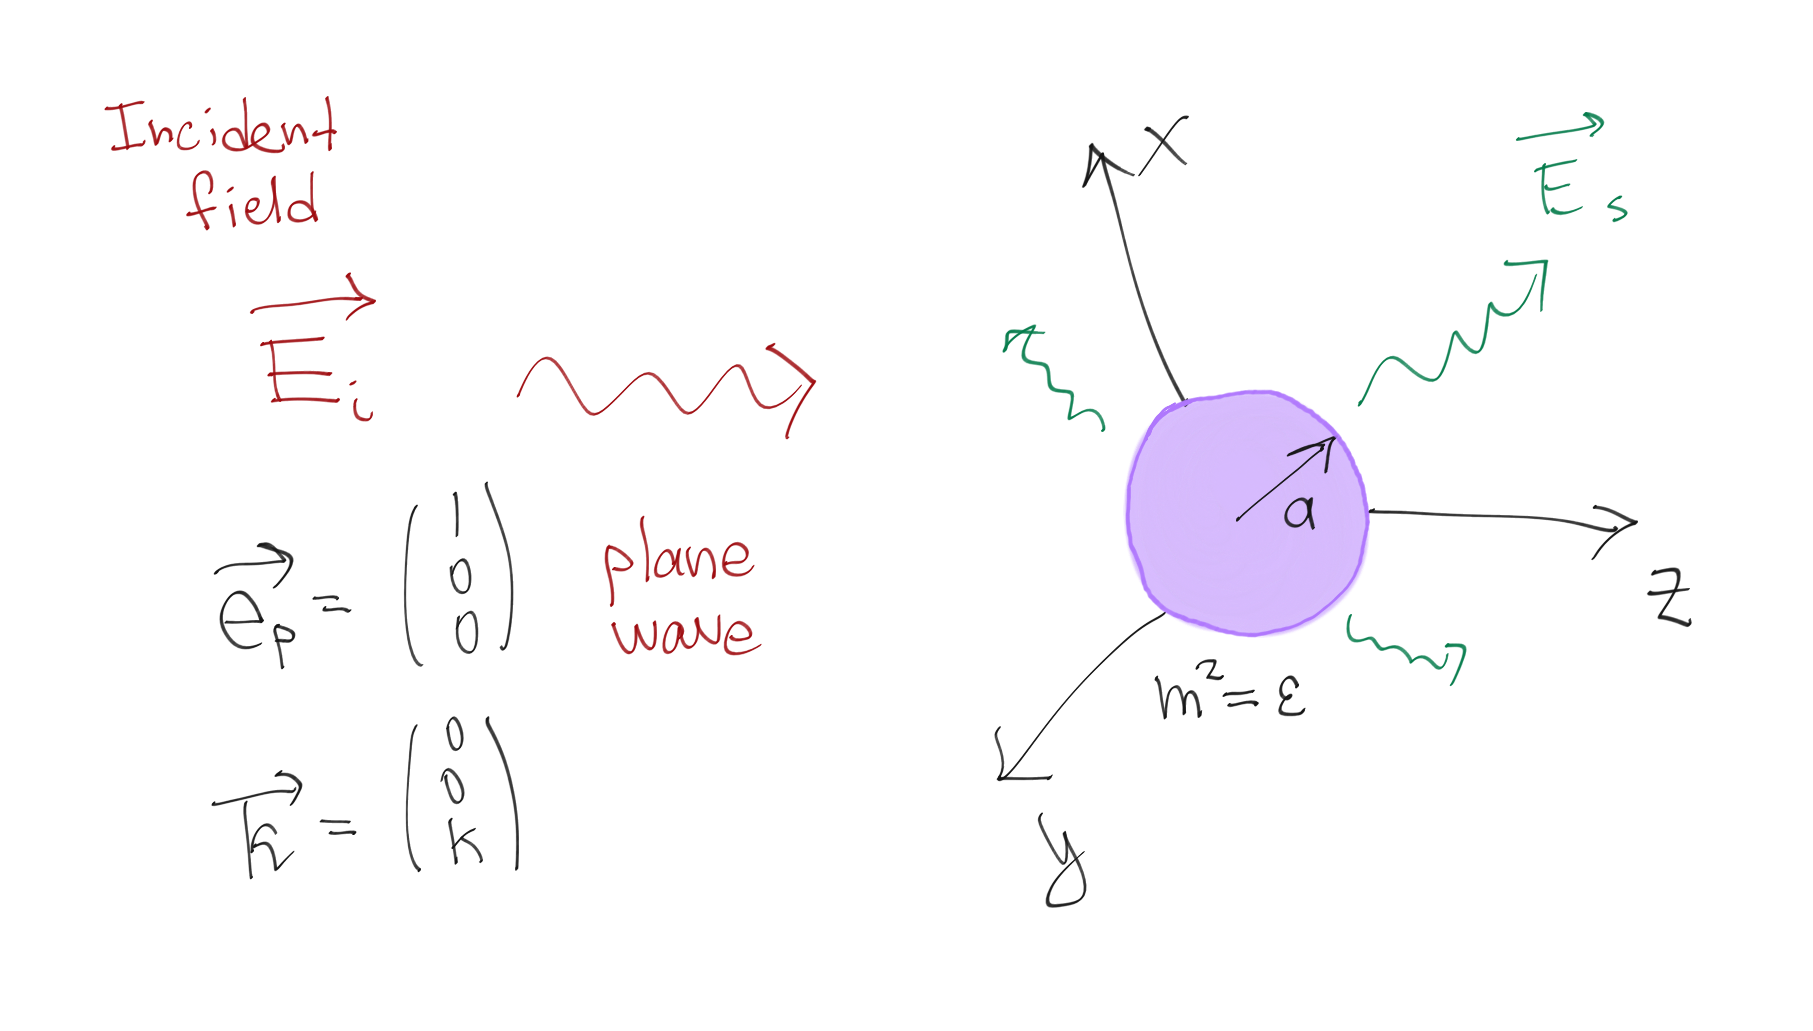
\includegraphics[width=0.83\linewidth]{../img/single_sph_scheme}\label{single_sph_scheme:image}\caption{Base model scheme.}
\end{tikzfigure}

Mie theory can be used to describe the scattered field and the field inside a scattering object. Consider a spherical cluster and $x$-polarized plane wave propagating along the $z$ axis (Fig.~\ref{single_sph_scheme:image}). Using generalized Fourier expansion in the case of an isotropic medium, we have the following form of the scattered field coefficients~\cite{boren_huffman}:

    \begin{equation}
		\vectbf{E}{s} = \sum_{n = 1}^{\infty}E_n \left[ i a_n\left(ka, m\right) \vectbf{N}{}^{(3)}_{e1n} - b_n\left(ka, m\right) \vectbf{M}{}^{(3)}_{o1n} \right], \quad E_n = i^{n} E_0 \frac{2n + 1}{n \left(n + 1\right)},
        \label{E_s_sph}
    \end{equation}

    \begin{equation}
		a_n(x,\:m) = \frac{m \func{\psi}{n}{\prime}{x} \func{\psi}{n}{}{mx} - \func{\psi}{n}{\prime}{mx} \func{\psi}{n}{}{x}}{m \func{\xi}{n}{\prime}{x} \func{\psi}{n}{}{mx} - \func{\psi}{n}{\prime}{mx} \func{\xi}{n}{}{x}},
		\label{an_bessel}
    \end{equation}

    \begin{equation}
        b_n(x,\:m) = \frac{\func{\psi}{n}{\prime}{x} \func{\psi}{n}{}{mx} - m \func{\psi}{n}{\prime}{mx} \func{\psi}{n}{}{x}}{\func{\xi}{n}{\prime}{x} \func{\psi}{n}{}{mx} - m \func{\psi}{n}{\prime}{mx} \func{\xi}{n}{}{x}},
        \label{bn_bessel}
    \end{equation}
    \begin{equation*} % artificial indent after the equation
    \end{equation*}

\noindent where $\funccomp{\psi}{n}{}{\rho} = z \funccomp{j}{n}{}{\rho}$, $\funccomp{\xi}{n}{}{\rho} = z \funccomp{h}{n}{}{\rho}$ --- Riccati-Bessel functions, $h_n = j_n + i \gamma_n$ --- spherical Hankel functions of the first kind, $x = ka$ --- dimensionless cluster radius, $ m = \sqrt{\varepsilon} $ --- complex refractive index.

% ============================= %

\begin{tikzfigure}
  \subcaptionbox{$ka = 0.5$, zero order approximation.}{
      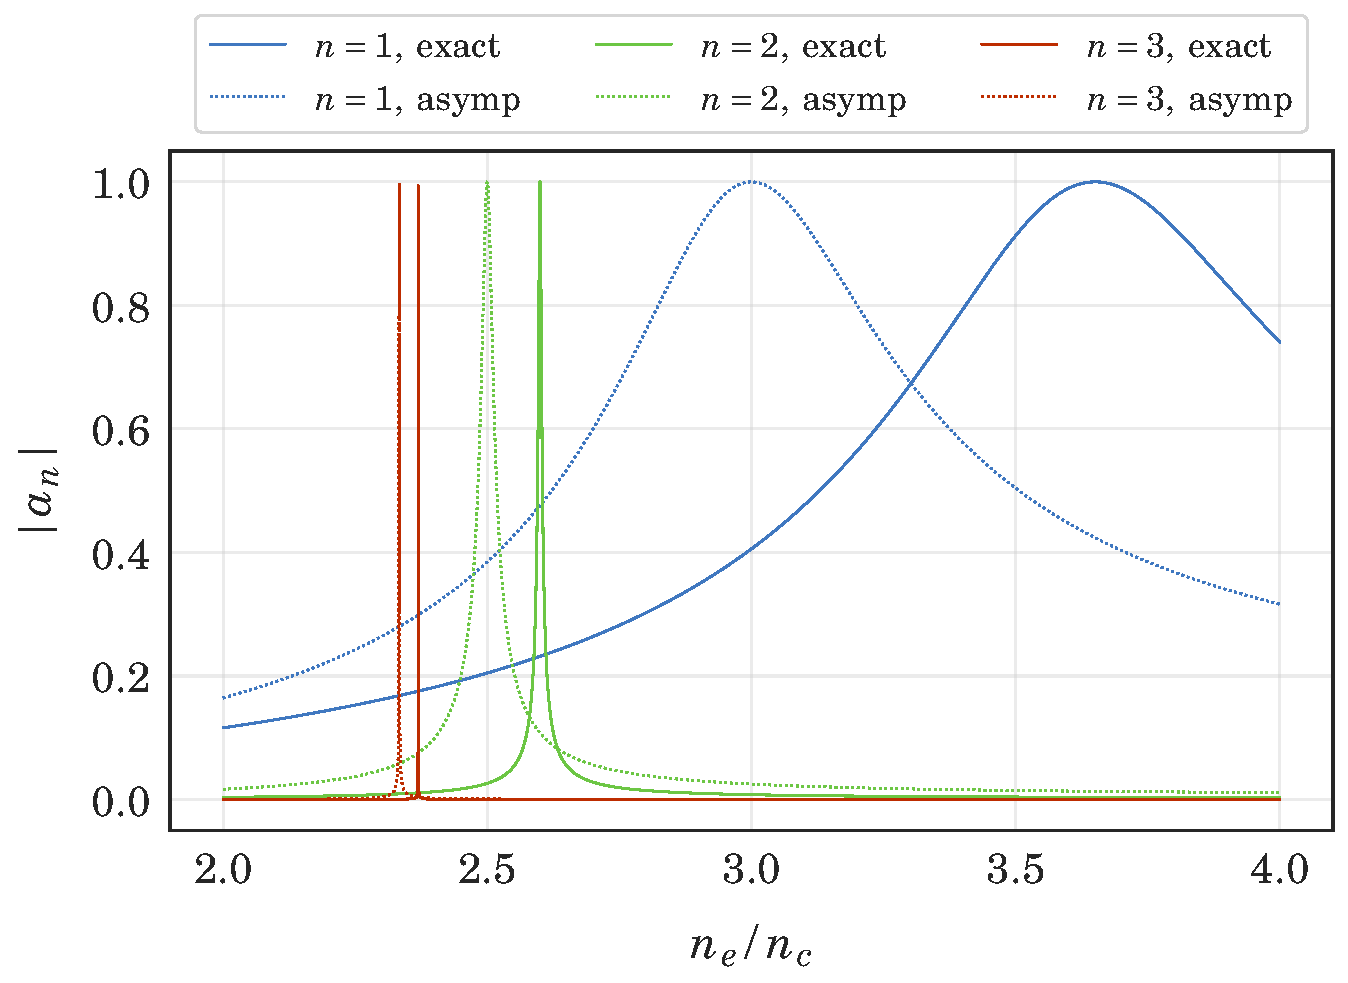
\includegraphics[width=0.48\linewidth]{../img/sph_base/sph_ka0.5_123}
  }
  \hfil
  \subcaptionbox{$ka = 1.5$, first order approximation.}{
      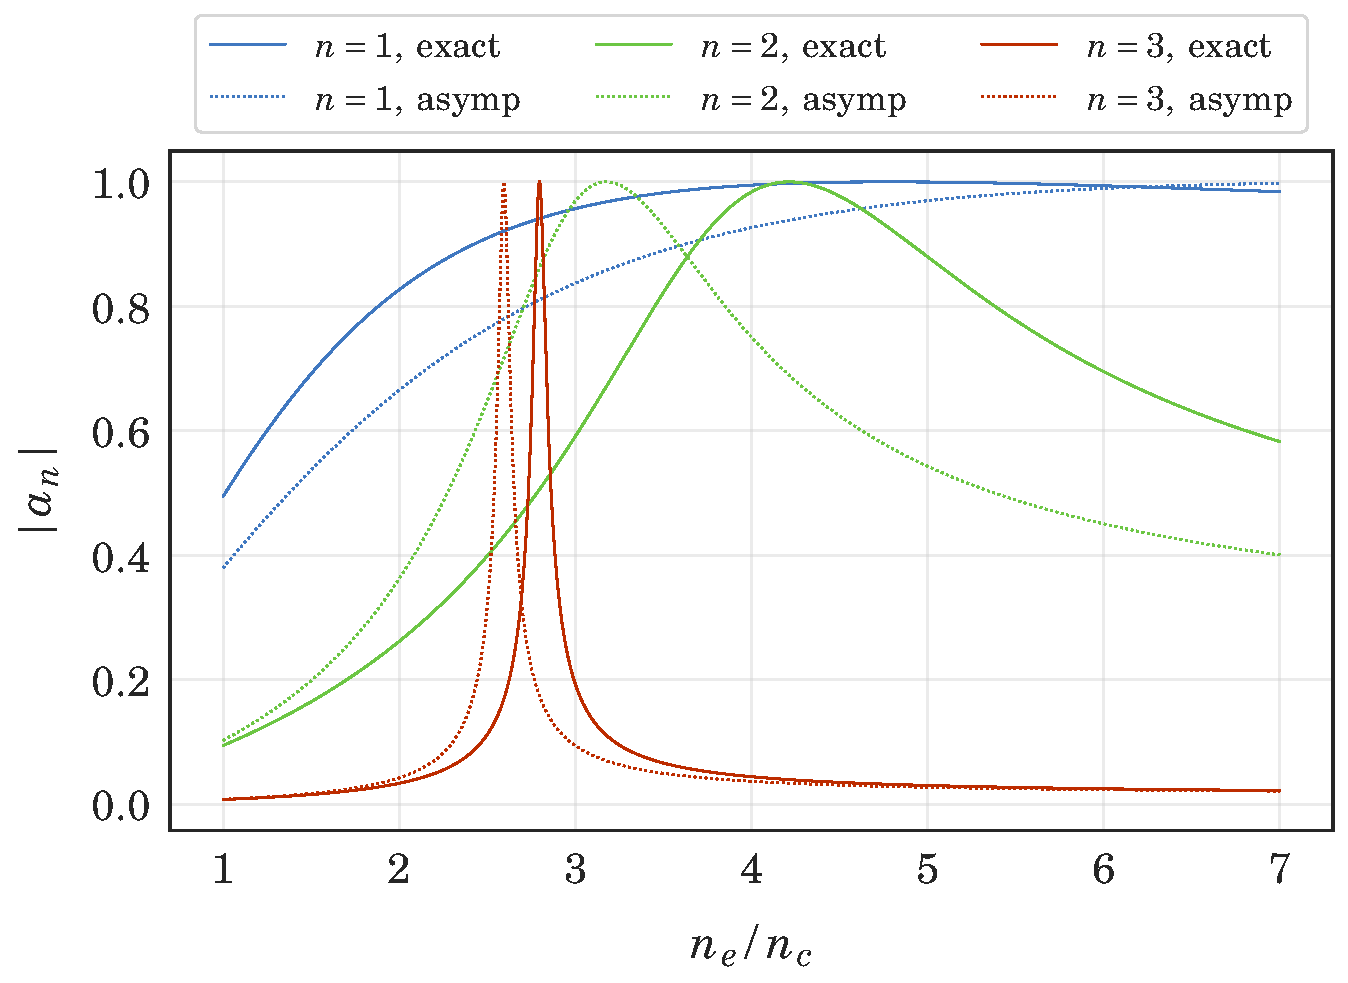
\includegraphics[width=0.48\linewidth]{../img/sph_base/sph_ka1.5_123_1st}
  }
  \label{ab_asymp:image}\caption{Coefficients of spherical harmonics in zero and first order approximation, $\beta_e = 0$. The ``exact'' curves are built using full expansions.}
\end{tikzfigure}